\documentclass[11pt,a4paper]{article}

\usepackage[utf8]{inputenc}
\usepackage[T1]{fontenc}
\usepackage[margin=2.5cm]{geometry}
\usepackage{hyperref}
\usepackage{booktabs}
\usepackage{longtable}
\usepackage{enumitem}
\usepackage{amsmath} 
\usepackage{listings}
\usepackage{xcolor}
\usepackage{graphicx}
\usepackage{tikz}
\usetikzlibrary{arrows.meta, positioning}

\hypersetup{
    colorlinks=true,
    linkcolor=blue,
    urlcolor=blue,
    citecolor=blue
}

\lstdefinestyle{javacode}{
    language=Java,
    basicstyle=\ttfamily\small,
    keywordstyle=\color{blue}\bfseries,
    commentstyle=\color{gray},
    stringstyle=\color{teal},
    numbers=left,
    numberstyle=\tiny\color{gray},
    stepnumber=1,
    numbersep=8pt,
    showstringspaces=false,
    breaklines=true,
    frame=single,
    rulecolor=\color{black!20},
    backgroundcolor=\color{black!3},
    tabsize=4,
    captionpos=b
}

\lstdefinestyle{properties}{
    language=,
    basicstyle=\ttfamily\small,
    numbers=left,
    numberstyle=\tiny\color{gray},
    breaklines=true,
    frame=single,
    rulecolor=\color{black!20},
    backgroundcolor=\color{black!3}
}

\title{VeriScreen Backend API\\Architecture and Implementation Guide}
\author{Sprint 1 --- Spring Boot 3.3 + JWT + PostgreSQL}
\date{\today}

\begin{document}

\maketitle
\tableofcontents
\newpage

%==============================================================================
\section{Introduction}
%==============================================================================

This document describes the \textbf{VeriScreen} Sprint~1 backend: a REST API built with \textbf{Spring Boot 3.3} (Java~17), \textbf{Spring Security}, \textbf{JWT} authentication, and \textbf{PostgreSQL}. There is no frontend in Sprint~1; the API is tested with Postman or similar tools.

\subsection{Goals}

\begin{itemize}[noitemsep]
    \item Authenticate students with student ID and password.
    \item Issue JWT tokens for stateless, session-free access.
    \item Expose protected endpoints for profile and document placeholders.
    \item Persist simulated university data in PostgreSQL.
\end{itemize}

\subsection{Technology Stack}

\begin{table}[h]
\centering
\begin{tabular}{@{}ll@{}}
\toprule
\textbf{Component} & \textbf{Choice} \\
\midrule
Framework       & Spring Boot 3.3.5 \\
Language        & Java 17 \\
Build tool      & Maven (\texttt{mvnw}) \\
Database        & PostgreSQL \\
ORM             & Spring Data JPA / Hibernate \\
Security        & Spring Security + JJWT 0.9.1 \\
Password hashing& BCrypt \\
API style       & REST (JSON), versioned \texttt{/api/v1} \\
API docs        & SpringDoc OpenAPI (\texttt{/swagger-ui.html}) \\
Default port    & 8080 \\
\bottomrule
\end{tabular}
\caption{Technology stack}
\end{table}

%==============================================================================
\section{Big Picture}
%==============================================================================

When the application starts, Spring Boot wires all components together. On first run, \textbf{mock student data} is inserted into the database. Clients interact as follows:

Both \textbf{legacy} (Sprint~1) and \textbf{versioned} URLs are supported:

\begin{table}[h]
\centering
\small
\begin{tabular}{@{}lll@{}}
\toprule
\textbf{Method} & \textbf{Legacy URL} & \textbf{Versioned URL} \\
\midrule
POST login & \texttt{/api/auth/login} & \texttt{/api/v1/auth/login} \\
GET profile & \texttt{/api/student/profile} & \texttt{/api/v1/students/me/profile} \\
GET documents & \texttt{/api/student/documents} & \texttt{/api/v1/students/me/documents} \\
\bottomrule
\end{tabular}
\caption{Supported API endpoints}
\end{table}

\begin{itemize}[noitemsep]
    \item Login must use \textbf{POST} with JSON body (GET returns 405).
    \item Protected routes require \texttt{Authorization: Bearer <token>}.
    \item Discovery: \texttt{GET /api/v1} lists endpoints (browser-friendly).
\end{itemize}

\subsection{Request Flow Diagram}

\begin{figure}[h]
\centering
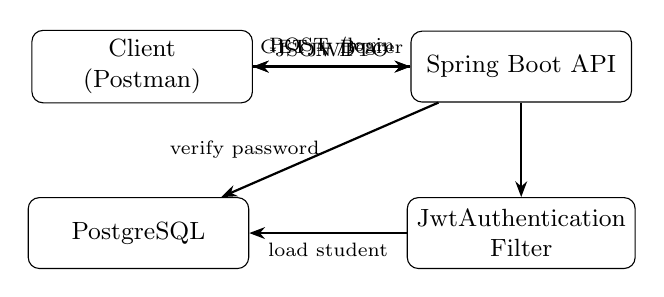
\begin{tikzpicture}[
    node distance=1.2cm and 2cm,
    box/.style={draw, rounded corners, minimum width=2.8cm, minimum height=0.9cm, align=center, font=\small},
    arrow/.style={-{Stealth[length=2mm]}, thick}
]
    \node[box] (client) {Client\\(Postman)};
    \node[box, right=of client] (api) {Spring Boot API};
    \node[box, below=of api] (filter) {JwtAuthentication\\Filter};
    \node[box, left=of filter] (db) {PostgreSQL};

    \draw[arrow] (client) -- node[above, font=\scriptsize]{POST /login} (api);
    \draw[arrow] (api) -- node[left, font=\scriptsize]{verify password} (db);
    \draw[arrow] (api) -- node[above, font=\scriptsize]{JWT} (client);

    \draw[arrow] (client) -- node[above, font=\scriptsize]{GET + Bearer} (api);
    \draw[arrow] (api) -- (filter);
    \draw[arrow] (filter) -- node[below, font=\scriptsize]{load student} (db);
    \draw[arrow] (api) -- node[above, font=\scriptsize]{JSON DTO} (client);
\end{tikzpicture}
\caption{High-level request flow for login and protected endpoints}
\end{figure}

\subsection{Login Sequence (Conceptual)}

\begin{enumerate}[noitemsep]
    \item Client sends student ID and plain-text password in JSON.
    \item \texttt{AuthController} delegates to \texttt{AuthService}.
    \item \texttt{AuthenticationManager} + \texttt{CustomUserDetailsService} verify credentials.
    \item BCrypt compares the submitted password with the stored hash.
    \item On success, \texttt{JwtService} signs a token with the student ID as subject.
    \item Client receives \texttt{\{ "accessToken": "..." \}}.
\end{enumerate}

\subsection{Protected Request Sequence (Conceptual)}

\begin{enumerate}[noitemsep]
    \item Client sends \texttt{Authorization: Bearer <token>}.
    \item \texttt{JwtAuthenticationFilter} extracts and validates the JWT.
    \item Valid token sets the authenticated user in \texttt{SecurityContextHolder}.
    \item Controller delegates to \texttt{StudentService} or \texttt{DocumentService}.
    \item \texttt{StudentAccessValidator} ensures the student accesses only their own data.
    \item Services use repositories; \texttt{StudentMapper} builds DTOs (no password in JSON).
\end{enumerate}

%==============================================================================
\section{Project Structure}
%==============================================================================

The main code lives under \texttt{src/main/java/com/veriscreen/backend/}.

\begin{table}[h]
\centering
\begin{tabular}{@{}lp{9cm}@{}}
\toprule
\textbf{Package} & \textbf{Role} \\
\midrule
\texttt{entity/}       & JPA entities (\texttt{@ManyToOne} to \texttt{Student}) \\
\texttt{repository/}  & Spring Data JPA (database only) \\
\texttt{dto/}          & API request/response JSON \\
\texttt{service/}      & \texttt{auth/}, \texttt{student/}, \texttt{document/}, \texttt{security/} \\
\texttt{mapper/}       & Entity $\rightarrow$ DTO mapping \\
\texttt{constants/}    & \texttt{ApiPaths} (single source for URLs) \\
\texttt{exception/}    & \texttt{GlobalExceptionHandler}, custom exceptions \\
\texttt{config/}       & Security, JWT filter, OpenAPI \\
\texttt{controller/}   & HTTP only (thin controllers) \\
\bottomrule
\end{tabular}
\caption{Package responsibilities}
\end{table}

\subsection{Dependency Injection}

Spring Boot uses \textbf{dependency injection} with \textbf{constructor injection}: controllers depend on service \textbf{interfaces} (\texttt{AuthService}, \texttt{StudentService}, \texttt{JwtService}), not concrete implementations. No \texttt{new} for services or repositories in application code.

%==============================================================================
\section{Configuration}
%==============================================================================

\subsection{application.properties}

File: \texttt{src/main/resources/application.properties}

\begin{lstlisting}[style=properties, caption={Application configuration (excerpt)}]
spring.application.name=veriscreen-backend

# PostgreSQL
spring.datasource.url=jdbc:postgresql://localhost:5432/veriscreen_db
spring.datasource.username=postgres
spring.datasource.password=<your-password>
spring.datasource.driver-class-name=org.postgresql.Driver

# JPA
spring.jpa.hibernate.ddl-auto=create-drop
spring.jpa.show-sql=true
spring.jpa.properties.hibernate.dialect=org.hibernate.dialect.PostgreSQLDialect

# JWT
jwt.secret=YourSuperSecretKeyAtLeast32CharactersLongChangeMe
jwt.expiration=86400000

# OpenAPI
springdoc.swagger-ui.path=/swagger-ui.html
\end{lstlisting}

\begin{table}[h]
\centering
\begin{tabular}{@{}lp{8.5cm}@{}}
\toprule
\textbf{Property} & \textbf{Meaning} \\
\midrule
\texttt{spring.datasource.*} & PostgreSQL connection URL, username, password \\
\texttt{ddl-auto=create-drop} & Hibernate creates tables on startup; drops them on shutdown (dev only) \\
\texttt{show-sql=true}        & Logs SQL statements to the console \\
\texttt{jwt.secret}            & Secret key used to sign and verify JWTs (keep private) \\
\texttt{jwt.expiration}        & Token lifetime in milliseconds (86400000 = 24 hours) \\
\bottomrule
\end{tabular}
\caption{Key configuration properties}
\end{table}

\subsection{Database Setup}

Before running the API, create the database:

\begin{lstlisting}[style=properties, caption={PostgreSQL}]
CREATE DATABASE veriscreen_db;
\end{lstlisting}

%==============================================================================
\section{Entities (Database Model)}
%==============================================================================

Each class annotated with \texttt{@Entity} maps to a database table. Lombok annotations (\texttt{@Data}, \texttt{@NoArgsConstructor}, \texttt{@AllArgsConstructor}) generate getters, setters, and constructors.

\subsection{Student}

Primary entity for authentication and profile. Table name: \texttt{students}.

\begin{itemize}[noitemsep]
    \item \texttt{id} (String, primary key) --- student number; also used as login username
    \item \texttt{name}, \texttt{nrc}, \texttt{program}, \texttt{enrollmentYear}
    \item \texttt{password} --- BCrypt-hashed; never returned in API responses
\end{itemize}

\subsection{Other Entities (Sprint 1: Schema Only)}

Repositories exist for future endpoints; Sprint~1 does not expose HTTP APIs for these yet.

\begin{table}[h]
\centering
\small
\begin{tabular}{@{}ll@{}}
\toprule
\textbf{Entity} & \textbf{Purpose} \\
\midrule
\texttt{Registration}     & Course registration records \\
\texttt{Fee}              & Fee payments and balances \\
\texttt{Examination}      & Exam eligibility and status \\
\texttt{AcademicResult}   & Course grades and credits \\
\texttt{HelsbApplication} & HELSB loan/scholarship applications \\
\bottomrule
\end{tabular}
\caption{Entities prepared for later sprints}
\end{table}

Child entities reference \texttt{Student} via \texttt{@ManyToOne(fetch = LAZY)} and \texttt{@JoinColumn(name = "student\_id")} instead of a loose string foreign key.

%==============================================================================
\section{Repositories}
%==============================================================================

Repository interfaces extend \texttt{JpaRepository<Entity, IdType>}. Spring generates implementations at runtime.

Example: \texttt{StudentRepository}

\begin{lstlisting}[style=javacode, caption={StudentRepository}]
@Repository
public interface StudentRepository extends JpaRepository<Student, String> {
}
\end{lstlisting}

Provided operations include \texttt{save()}, \texttt{findById()}, \texttt{count()}, \texttt{delete()}, and more, without writing SQL manually.

%==============================================================================
\section{DTOs (Data Transfer Objects)}
%==============================================================================

DTOs define the JSON shape exposed to clients and hide sensitive entity fields.

\begin{table}[h]
\centering
\begin{tabular}{@{}lp{7.5cm}@{}}
\toprule
\textbf{Class} & \textbf{Usage} \\
\midrule
\texttt{LoginRequest}      & Request body for login: \texttt{id}, \texttt{password} \\
\texttt{JwtResponse}       & Response: \texttt{accessToken} \\
\texttt{StudentProfileDto} & Profile response: id, name, program, enrollmentYear (no password) \\
\texttt{DocumentDto}       & Document list items: type, url, generatedDate \\
\bottomrule
\end{tabular}
\caption{DTO classes}
\end{table}

%==============================================================================
\section{Security Architecture}
%==============================================================================

\subsection{SecurityConfig}

Class: \texttt{config/SecurityConfig.java}

\begin{lstlisting}[style=javacode, caption={Security filter chain (excerpt)}]
http.csrf(csrf -> csrf.disable())
    .authorizeHttpRequests(auth -> auth
        .requestMatchers("/api/v1", "/api/v1/auth/login",
            "/api/auth/login", "/swagger-ui/**", "/v3/api-docs/**")
        .permitAll()
        .anyRequest().authenticated())
    .sessionManagement(session -> session
        .sessionCreationPolicy(SessionCreationPolicy.STATELESS));

http.authenticationProvider(authenticationProvider());
http.addFilterBefore(jwtAuthenticationFilter,
    UsernamePasswordAuthenticationFilter.class);
\end{lstlisting}

\begin{itemize}[noitemsep]
    \item Public: login URLs, \texttt{GET /api/v1} discovery, Swagger/OpenAPI.
    \item All other routes --- must be authenticated.
    \item \texttt{STATELESS} --- no HTTP sessions; identity comes from JWT on each request.
    \item CSRF disabled --- common for stateless REST APIs using JWT.
    \item \texttt{BCryptPasswordEncoder} --- hashes passwords on save; verifies on login.
\end{itemize}

\subsection{CustomUserDetailsService}

Class: \texttt{service/CustomUserDetailsService.java}

Implements Spring Security's \texttt{UserDetailsService}:

\begin{enumerate}[noitemsep]
    \item Receives username (student \texttt{id}).
    \item Loads \texttt{Student} from \texttt{StudentRepository}.
    \item Builds a Spring \texttt{User} with username = id and password = hash from DB.
    \item Used during login (password check) and when the JWT filter reloads the user.
\end{enumerate}

\subsection{JwtService (interface) and JwtServiceImpl}

Interface: \texttt{service/security/JwtService.java}. Implementation: \texttt{JwtServiceImpl} (JWT only; no database access).

\begin{table}[h]
\centering
\begin{tabular}{@{}lp{8cm}@{}}
\toprule
\textbf{Method} & \textbf{Behavior} \\
\midrule
\texttt{generateToken(studentId)}  & Builds signed JWT; subject = student ID; expiry from config \\
\texttt{extractStudentId(token)}   & Parses token and returns subject (student ID) \\
\texttt{validateToken(token)}      & Returns true if signature valid and not expired \\
\bottomrule
\end{tabular}
\caption{JwtService methods}
\end{table}

\subsection{JwtAuthenticationFilter}

Class: \texttt{config/JwtAuthenticationFilter.java}

Extends \texttt{OncePerRequestFilter} --- runs once per HTTP request, before controllers.

\begin{lstlisting}[style=javacode, caption={JWT filter logic (excerpt)}]
final String authHeader = request.getHeader("Authorization");
if (authHeader == null || !authHeader.startsWith("Bearer ")) {
    chain.doFilter(request, response);
    return;
}
String token = authHeader.substring(7);
String studentId = jwtService.extractStudentId(token);
if (studentId != null && SecurityContextHolder.getContext().getAuthentication() == null) {
    UserDetails userDetails = userDetailsService.loadUserByUsername(studentId);
    if (jwtService.validateToken(token)) {
        UsernamePasswordAuthenticationToken authToken =
            new UsernamePasswordAuthenticationToken(
                userDetails, null, userDetails.getAuthorities());
        SecurityContextHolder.getContext().setAuthentication(authToken);
    }
}
chain.doFilter(request, response);
\end{lstlisting}

If the header is missing on a protected route, the filter passes through and Spring Security returns \textbf{401 Unauthorized}.

%==============================================================================
\section{REST Controllers}
%==============================================================================

\subsection{AuthController}

Base paths: \texttt{/api/v1/auth} and \texttt{/api/auth} (legacy). Delegates to \texttt{AuthService}; no business logic in controller.

\begin{lstlisting}[style=javacode, caption={Login endpoint (excerpt)}]
@PostMapping("/login")
public ResponseEntity<JwtResponse> login(@RequestBody @Valid LoginRequest request) {
    return ResponseEntity.ok(authService.login(request));
}
\end{lstlisting}

\subsection{StudentController and LegacyStudentController}

\begin{itemize}[noitemsep]
    \item \texttt{StudentController}: \texttt{/api/v1/students/me/profile}, \texttt{/me/documents}, and \texttt{/\{studentId\}/...} with ownership checks.
    \item \texttt{LegacyStudentController}: \texttt{/api/student/profile} and \texttt{/api/student/documents}.
    \item Controllers call \texttt{StudentService} and \texttt{DocumentService} only.
\end{itemize}

\subsection{DocumentGenerator (Open/Closed)}

New document types (e.g.\ transcript) are added by implementing \texttt{DocumentGenerator} and registering with \texttt{@Component}. \texttt{DocumentServiceImpl} collects all generators automatically; existing code is not modified.

%==============================================================================
\section{DataLoader (Mock Data)}
%==============================================================================

Class: \texttt{service/DataLoader.java}

Implements \texttt{CommandLineRunner} --- executes after application startup.

\begin{itemize}[noitemsep]
    \item If \texttt{studentRepository.count() == 0}, inserts one test student.
    \item ID: \texttt{2021465934}, name: Samuel Mwanza, program: Computer Science.
    \item Password \texttt{password123} is encoded with BCrypt before \texttt{save()}.
\end{itemize}

This enables immediate Postman testing without manual SQL inserts.

%==============================================================================
\section{Application Entry Point}
%==============================================================================

Class: \texttt{BackendApplication.java}

\begin{lstlisting}[style=javacode, caption={Main class}]
@SpringBootApplication
public class BackendApplication {
    public static void main(String[] args) {
        SpringApplication.run(BackendApplication.class, args);
    }
}
\end{lstlisting}

\texttt{@SpringBootApplication} enables auto-configuration, component scanning under \texttt{com.veriscreen.backend}, and embedded Tomcat on port 8080.

%==============================================================================
\section{Building and Running}
%==============================================================================

\begin{lstlisting}[style=properties, caption={Commands (Windows)}]
cd backend
mvnw.cmd clean install -DskipTests
mvnw.cmd spring-boot:run
\end{lstlisting}

API base URL: \url{http://localhost:8080}

%==============================================================================
\section{Postman Testing}
%==============================================================================

\subsection{Login}

\begin{table}[h]
\centering
\begin{tabular}{@{}ll@{}}
\toprule
\textbf{Field} & \textbf{Value} \\
\midrule
Method  & POST \\
URL     & \texttt{http://localhost:8080/api/auth/login} \\
Headers & \texttt{Content-Type: application/json} \\
Body    & \texttt{\{"id":"2021465934","password":"password123"\}} \\
\bottomrule
\end{tabular}
\caption{Login request}
\end{table}

Expected response:

\begin{lstlisting}[style=properties]
{
  "accessToken": "eyJhbGciOiJIUzI1NiJ9..."
}
\end{lstlisting}

\subsection{Get Profile}

\begin{table}[h]
\centering
\begin{tabular}{@{}ll@{}}
\toprule
\textbf{Field} & \textbf{Value} \\
\midrule
Method  & GET \\
URL     & \texttt{http://localhost:8080/api/student/profile} \\
Headers & \texttt{Authorization: Bearer <paste-token-here>} \\
\bottomrule
\end{tabular}
\caption{Profile request}
\end{table}

\subsection{Get Documents}

Same as profile, but URL: \texttt{http://localhost:8080/api/student/documents}.

\subsection{Troubleshooting}

\begin{table}[h]
\centering
\small
\begin{tabular}{@{}lll@{}}
\toprule
\textbf{Error} & \textbf{Cause} & \textbf{Fix} \\
\midrule
403 on login & Protected URL or token sent on login & Use login URL; Authorization = No Auth \\
405 on login & GET instead of POST & Use POST + JSON body \\
401 on profile & Missing/invalid JWT & Login first; Bearer token in header \\
\bottomrule
\end{tabular}
\caption{Common Postman issues}
\end{table}

See also \texttt{docs/CODE\_REVIEW\_CHECKLIST.md} for pre-commit quality checks.

%==============================================================================
\section{Sprint 1 Checklist}
%==============================================================================

\begin{table}[h]
\centering
\begin{tabular}{@{}lc@{}}
\toprule
\textbf{Item} & \textbf{Status} \\
\midrule
PostgreSQL database created and connected & User setup \\
All entities and repositories exist     & Done \\
JWT generation and validation           & Done \\
Login returns token with valid credentials& Done \\
Protected profile requires valid token    & Done \\
Mock data loads on startup                & Done \\
Endpoints tested in Postman               & User testing \\
Code committed to Git                     & Done \\
\bottomrule
\end{tabular}
\caption{Sprint 1 completion checklist}
\end{table}

%==============================================================================
\section{Out of Scope for Sprint 1}
%==============================================================================

\begin{itemize}
    \item HTTP endpoints for registrations, fees, examinations, academic results, HELSB.
    \item Real document generation (PDFs); \texttt{/documents} returns static placeholders.
    \item Refresh tokens, password reset, role-based access (admin vs student).
    \item Production-ready DDL strategy (\texttt{create-drop} wipes schema on shutdown).
    \item Frontend application.
\end{itemize}

%==============================================================================
\section{Summary}
%==============================================================================

\textbf{One-sentence model:} PostgreSQL stores students; login verifies BCrypt and returns a JWT; every protected request validates the JWT in a filter; thin controllers delegate to services, which return DTOs without passwords.

\vspace{1em}
\noindent\textbf{Layer flow:}
\[
\text{HTTP} \rightarrow \text{JwtAuthenticationFilter} \rightarrow \text{Controller}
\rightarrow \text{Service} \rightarrow \text{Repository} \rightarrow \text{PostgreSQL}
\]

\end{document}
